\subsection{Ansteuerung BLDC Motor}
\label{sec:bldc}
Die Ansteuerung für den BLDC Motor\footnote{\textbf{B}rush\textbf{L}ess 
\textbf{D}irect \textbf{C}urrent Motor} wird in in der Gruppe PREN-ET 
entwickelt. (Siehe \ref{sec:pren-et} \nameref{sec:pren-et}) 
%Daher werden hier nur Anpassungen für das Team 27 betrachtet. 
\begin{figure}[h!]
    \centering
    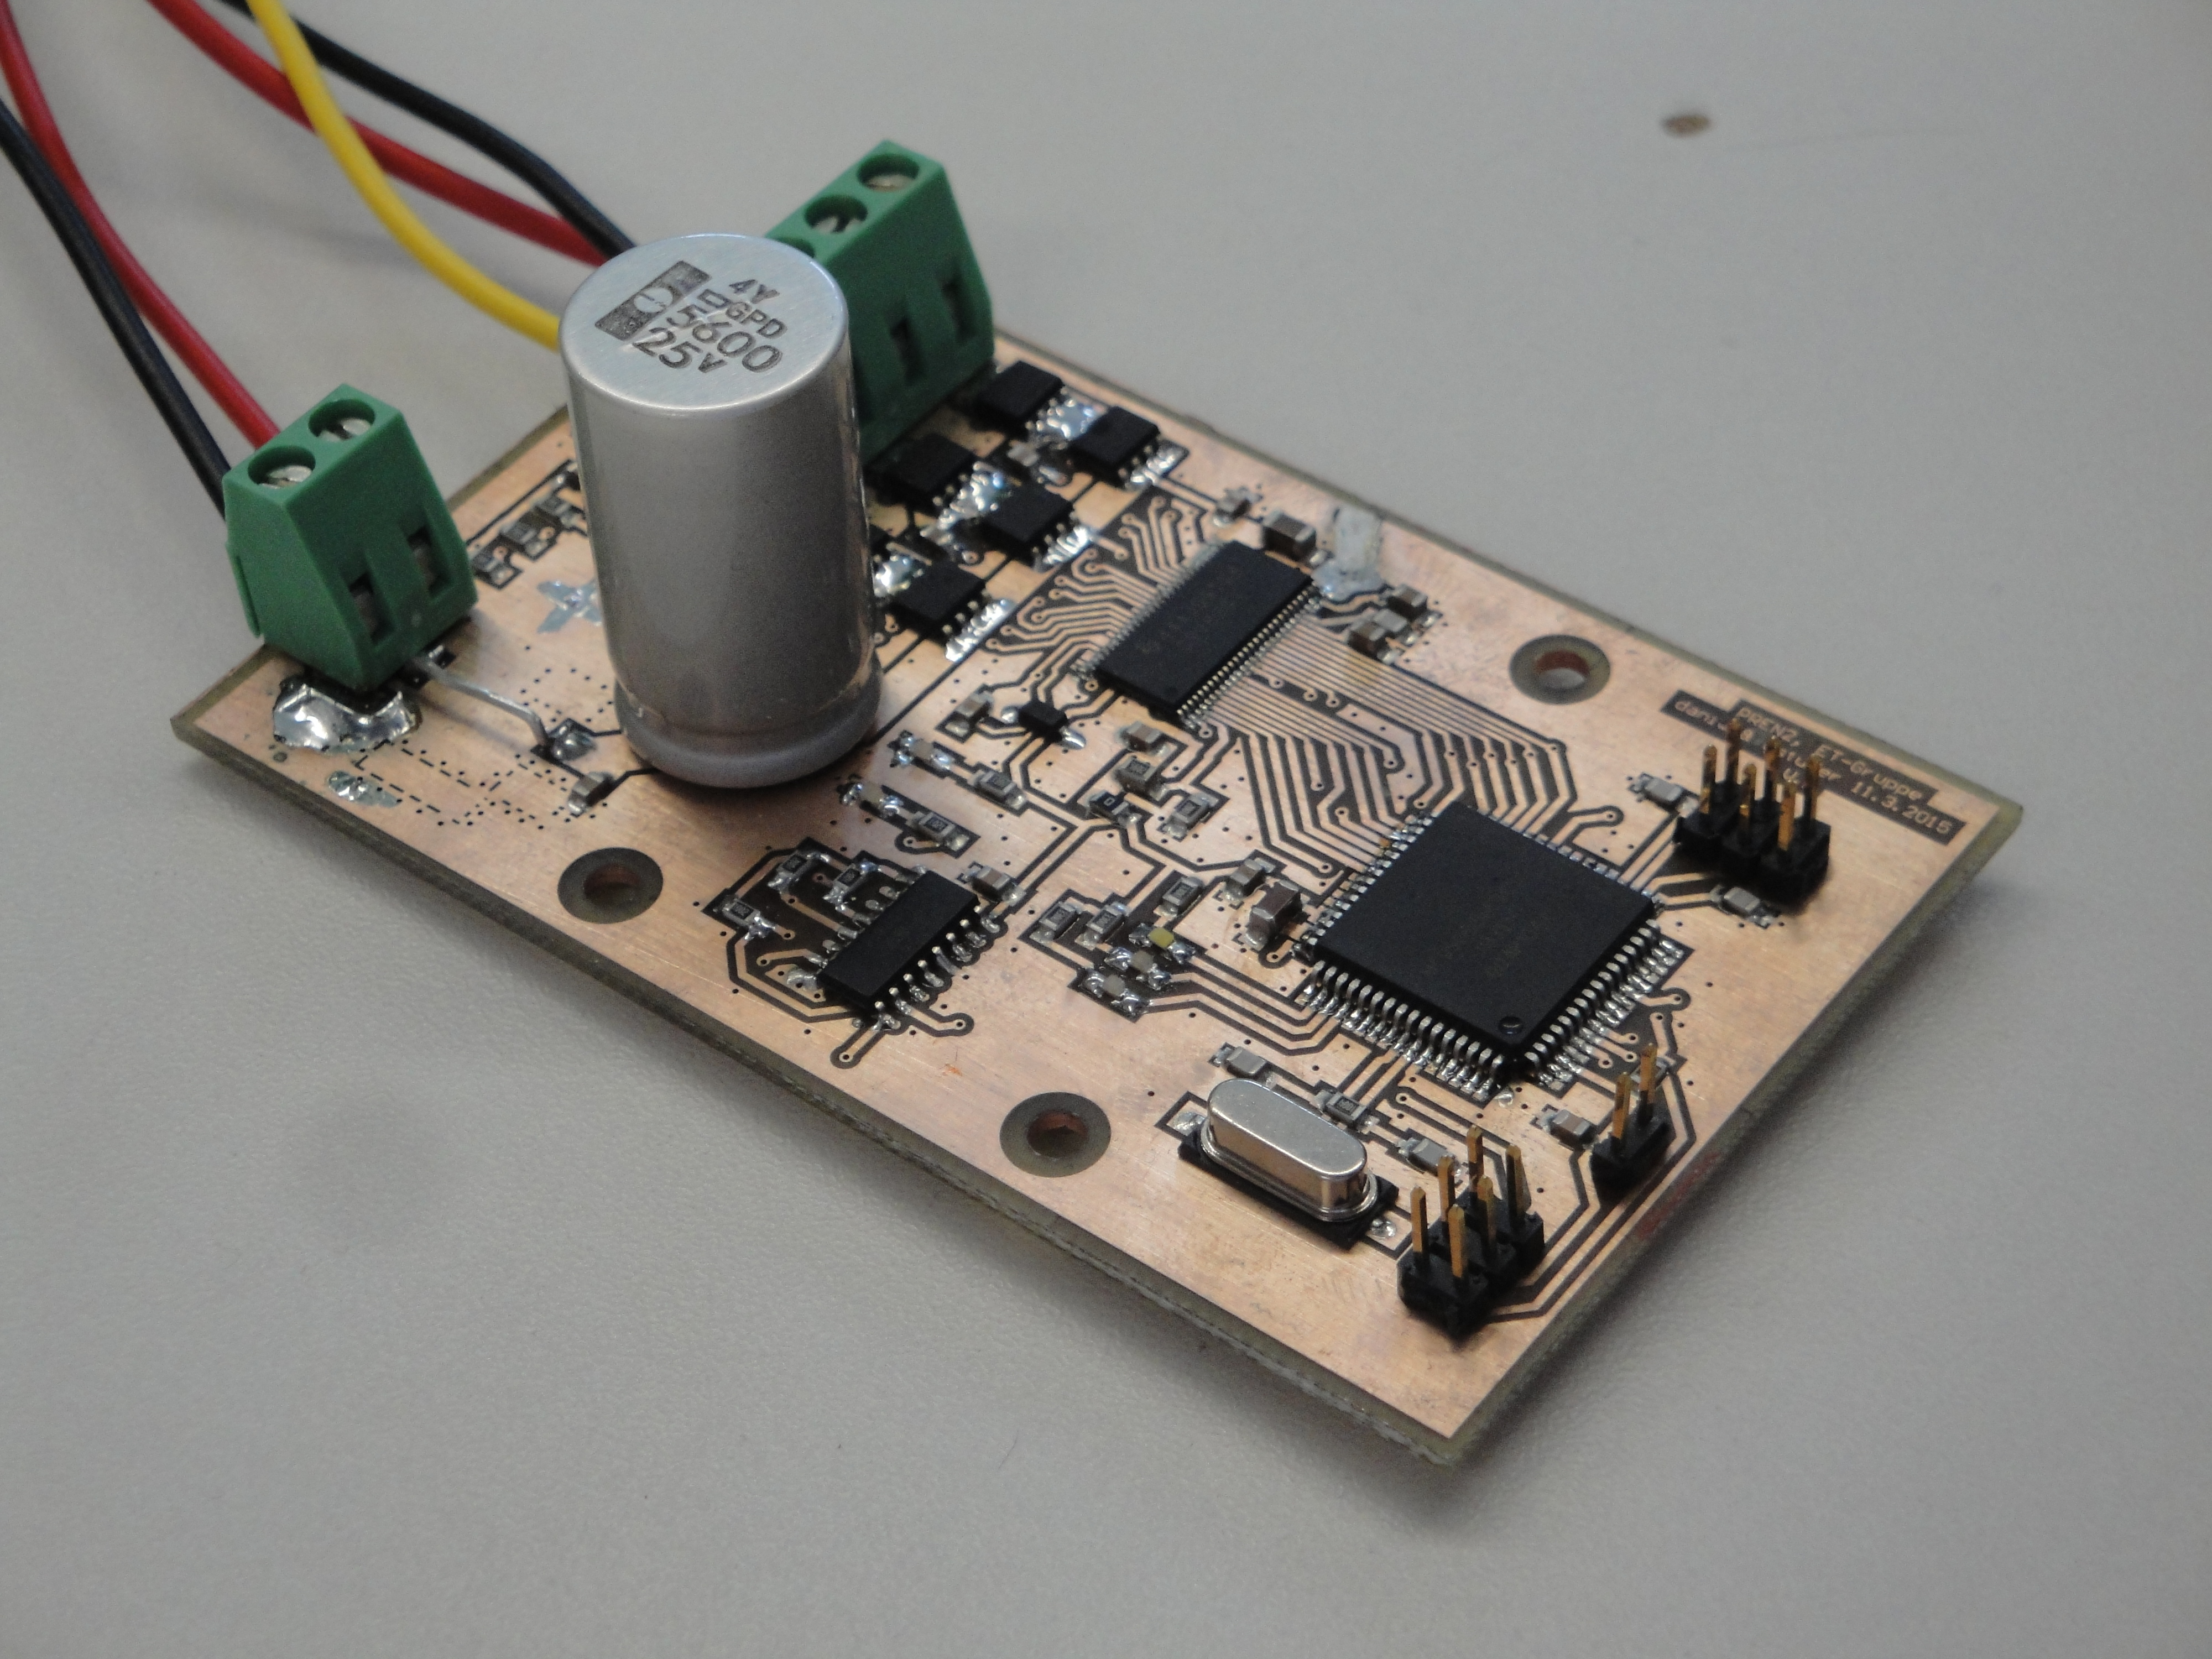
\includegraphics[width=0.7\textwidth]{fig_pcb/DSC02906.JPG}
    \caption{Ansteuerung BLDC Motor}
    \label{fig:dc}
\end{figure}

\noindent
Die Ansteuerung für den BLDC Motor übernimmt die Kommutierung des Motors und 
die Regelung der Drehzahl. Für die korrekte Kommutierung ist es notwendig, die 
aktuelle Position des Rotors zu kennen. Es wird eine sensorlose Kommutierung 
verwendet. Das bedeutet, dass keine Sensoren für die Rückmeldung der aktuellen 
Rotorposition notwendig sind. Stattdessen wird die Position aus der 
induzierten Spannung der nicht bestromten Phase bestimmt. Diese Detektion 
funktioniert jedoch nur bei drehendem Motor. Daher muss der Motor mit 
Zwangskommutierung gestartet werden. Nach dem Starten des Motors wird der 
Regler aktiviert, welcher für eine konstante Drehzahl des Motors sorgt. Als 
Regler kommt ein PID-Regler mit Stellgrössenbegrenzung zum Einsatz. Da die 
Ansteuerung und die Regelung komlett selbst in der Gruppe PREN-ET entwickelt 
wird, besteht Zugriff auf alle relevanten Regelparameter. Zudem kann mit dem 
Motor das Endsignal ausgegeben werden. 
